\documentclass[12pt]{article}
\usepackage[utf8x]{inputenc}
\usepackage{amsmath}
\usepackage{graphicx}
\usepackage{float}
\usepackage{dsfont}
\usepackage{amsfonts}
\usepackage[T1]{fontenc}
\usepackage[colorinlistoftodos]{todonotes}
\usepackage[margin=2.5cm,a4paper]{geometry}
\usepackage{listings}
\usepackage{minted}
\usepackage{multicol}
\usepackage{fancyhdr}
\usepackage{cite}
\usepackage{cleveref}
\usepackage{siunitx}
\setlength{\parindent}{0pt}
\newcommand{\deriv}{\mathrm{d}}
\lstset{
    language=R,
    basicstyle=\scriptsize\ttfamily,
    commentstyle=\ttfamily\color{red},
    numbers=left,
    numberstyle=\ttfamily\color{blue}\footnotesize,
    stepnumber=1,
    numbersep=5pt,
    backgroundcolor=\color{white},
    showspaces=false,
    showstringspaces=false,
    showtabs=false,
    frame=single,
    tabsize=2,
    captionpos=b,
    breaklines=true,
    breakatwhitespace=false,
    title=\lstname,
    escapeinside={},
    keywordstyle={},
    morekeywords={}
    }

\pagestyle{fancy}
\fancyhf{}
\rhead{PH370 Physics Labs}
\lhead{Investigating diodes \& rectification of an AC signal}
\rfoot{-\thepage\centering-}

\begin{document}
\begin{titlepage}

\newgeometry{left=1.5in,right=1.5in,top=2.5in,bottom=2.5in}
\newcommand{\HRule}{\rule{\linewidth}{0.5mm}}

\begin{centering} 
 
%------------------------------------------------------------------------
%	HEADING SECTIONS
%------------------------------------------------------------------------


\includegraphics[scale=0.4]{Uni_of_Kent_Logo.png}\\[1cm]

%------------------------------------------------------------------------
%	TITLE SECTION
%------------------------------------------------------------------------

\HRule \\[0.4cm]
\textsc{\large Astronomy, Space Science and Astrophysics}\\[0.4cm]
{\huge \bfseries Investigating diodes \& \\ [0.4cm] rectification of an AC signal}\\[0.4cm]
\HRule \\[1.0cm]

%------------------------------------------------------------------------
%	DATE SECTION
%------------------------------------------------------------------------

\textsc{\Large Stage 1 - PH370 Physics Labs}\\[0.5cm] 
{\large Monday 15th/22nd January 2017}\\[1.0cm]

%------------------------------------------------------------------------
%	AUTHOR SECTION
%------------------------------------------------------------------------

\begin{minipage}{0.625\textwidth}
\centering

\emph{\large Report Author:} \large Lukasz R Tomaszewski \\ [0.2cm]
\emph{\large Lab Partner:} \large Benedict John Wye \\

\end{minipage}\\[2cm]

\vfill
\end{centering} 
\end{titlepage}

%------------------------------------------------------------------------
%------------------------------------------------------------------------
%	CONTENTS  
%------------------------------------------------------------------------
%------------------------------------------------------------------------

\newpage
\begin{titlepage}
\begin{tableofcontents}

\end{tableofcontents}
\end{titlepage}

%-----------------------------------------------------------------------
%-----------------------------------------------------------------------
%	INTRODUCTION   
%-----------------------------------------------------------------------
%-----------------------------------------------------------------------

\section{Introduction}

Diodes are electronic components which allow current to only flow in one direction. Within this experiment, i will explore the properties of various diodes (As can be seen in \cref{SymbolRegDiode}). 

\begin{figure}[h]
\centering
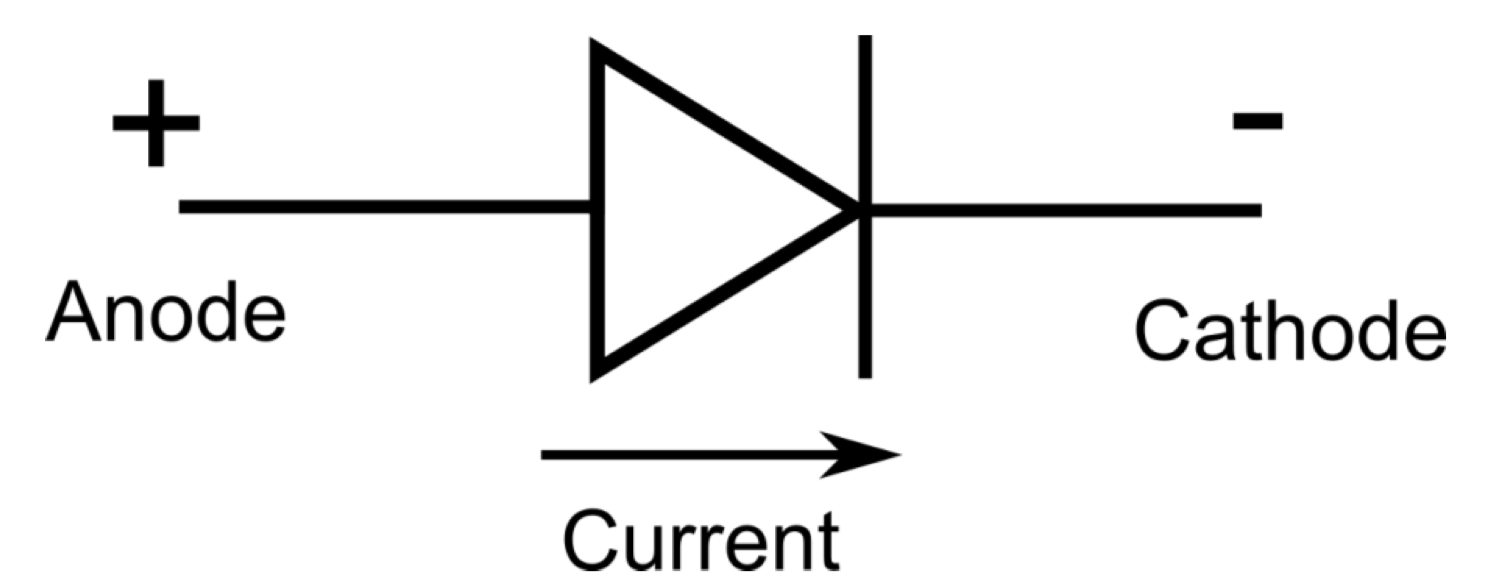
\includegraphics[scale=0.4]{Circuit_symbol_for_a_regular_diode.png}
\caption{Circuit symbol for a regular diode.}
\label{SymbolRegDiode}
\end{figure}

The 

%-----------------------------------------------------------------------
%-----------------------------------------------------------------------
%	METHOD & EQUIPMENT
%-----------------------------------------------------------------------
%-----------------------------------------------------------------------

\section{Method \& Equipment}

%-----------------------------------------------------------------------
%	APPARTUS 
%-----------------------------------------------------------------------

\subsection{Apparatus}

\begin{multicols}{2}
\begin{itemize}
	\item Oscilloscope
    \item Signal generator
    \item Electronic components \begin{itemize}
    \item 470 {\si{\ohm}} Resistor
    \item 1 k{\si{\ohm}} Resistor
    \item 10 k{\si{\ohm}} Resistor
    \item 1 {\si{\mu}}F Capacitor
    \item 10 {\si{\mu}}F Capacitor 
    \end{itemize}
    \item 3 x BNC Lead
    \item Leybold Plug-in board
    \item 2 x Banana plugs to BNC socket
    \item Diodes \begin{itemize}
    \item 1N4007 Diode
    \item Red \& Blue LED's
    \item 3.3V Zener Diode
    \end{itemize}
\end{itemize}
\end{multicols}

%-----------------------------------------------------------------------
%	DATA COLLECTED
%-----------------------------------------------------------------------

\subsection{Data Collected}

\begin{multicols}{2}
\begin{itemize}
	\item f
\end{itemize}
\end{multicols}

%-----------------------------------------------------------------------
%	RISK ASSESSMENT
%-----------------------------------------------------------------------

\subsection{Risk Assessment}

efwfwef

%-----------------------------------------------------------------------
%-----------------------------------------------------------------------
%	EXPERIMENTAL PROCEDURE
%-----------------------------------------------------------------------
%-----------------------------------------------------------------------

\section{Experimental Procedure}

%-----------------------------------------------------------------------
%	RELATIONSHIP BETWEEN VOLTAGE AND CURRENT FOR A DIODE
%-----------------------------------------------------------------------

\subsection{Relationship between voltage and current for a diode}

s

\begin{figure}[h]
\centering
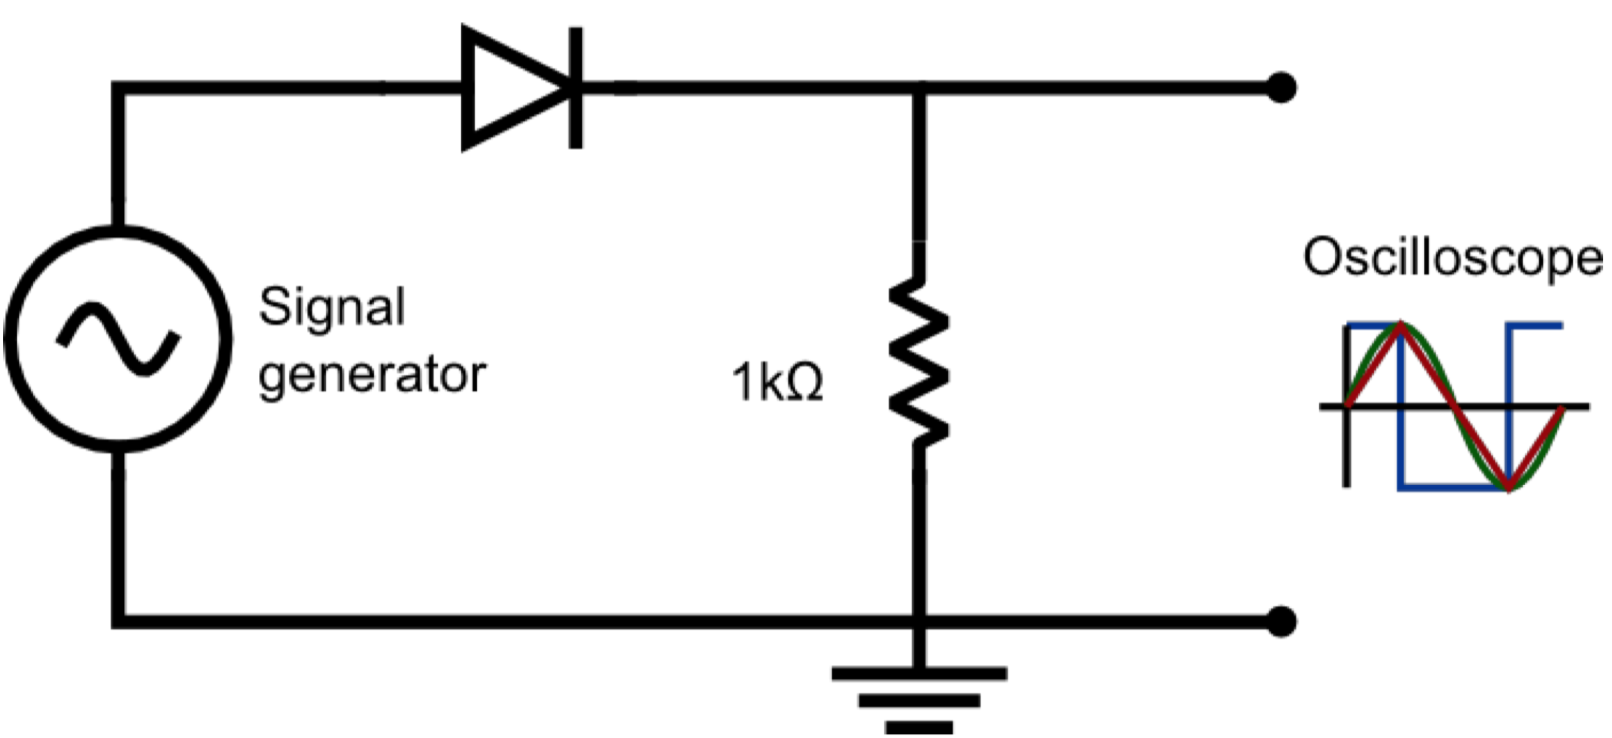
\includegraphics[scale=0.35]{Half_Wave_Retification.png}
\caption{Circuit for half-wave rectification.}
\label{SymbolHalfWaveRet}
\end{figure}

%-----------------------------------------------------------------------
%	HALF-WAVE RETIFICATION OF AN AC SIGNAL
%-----------------------------------------------------------------------

\subsection{Half-wave rectification of an AC signal}

%-----------------------------------------------------------------------
%	INVESTIGATING THE CHARACTERISTICS OF LEDS
%-----------------------------------------------------------------------

\subsection{Investigating the Characteristics of LEDs}

%-----------------------------------------------------------------------
%	LEDS IN PARALLEL
%-----------------------------------------------------------------------

\subsection{LEDs in parallel}

%-----------------------------------------------------------------------
%	DIM LEDS: AN INTRODUCTION TO PULSE WIDTH MODULATION (PWM)
%-----------------------------------------------------------------------

\subsection{Dim LEDs: An Introduction to Pulse Width Modulation (PWM)}

%-----------------------------------------------------------------------
%	USING A ZENER DIODE AS VOLTAGE REGULATOR
%-----------------------------------------------------------------------

\subsection{Using a Zener diode as voltage regulator}

%-----------------------------------------------------------------------
%-----------------------------------------------------------------------
%	RESULT & DISSCUSSION
%-----------------------------------------------------------------------
%-----------------------------------------------------------------------

\section{Results \& Disscussion}

%-----------------------------------------------------------------------
%	MAIN RESULTS
%-----------------------------------------------------------------------

\subsection{Main Results}

\begin{tabular}{l*{6}{c}r}
Input Voltage    200mv & 300mv & 400mv & 500mv & 600mv & 700mv & 800mv & 900mv \\
\hline
Output Voltage   & 6 & 4 & 0 & 2 & 10 & 5 & 12  \\
\\

\end{tabular}

%-----------------------------------------------------------------------
%	ANALYSIS
%-----------------------------------------------------------------------

\subsection{Analysis}

%-----------------------------------------------------------------------
%-----------------------------------------------------------------------
%	CONCLUSION
%-----------------------------------------------------------------------
%-----------------------------------------------------------------------

\section{Conclusion}

%------------------------------------------------------------------------
%	REFERENCES
%------------------------------------------------------------------------

\bibliographystyle{plain}

%------------------------------------------------------------------------

\pagebreak
\inputminted[breaklines]{tex}{main.tex}

\end{document}